\begin{figure*}
  \centering
  \begin{subfigure}[b]{0.05\textwidth}
    ~
  \end{subfigure}
  \hfill
  \begin{subfigure}[b]{0.3\textwidth}
    \centering
    ~~~~~\textbf{Random layout}
  \end{subfigure}
  \hfill 
  \begin{subfigure}[b]{0.3\textwidth}
    \centering
    ~~~~~~\textbf{PLAID layout}
  \end{subfigure}
  \hfill
  \begin{subfigure}[b]{0.3\textwidth}
    \centering
    ~~~~~~\textbf{COMPD layout}
  \end{subfigure}



  \begin{subfigure}[c]{0.05\textwidth}
    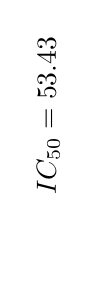
\begin{tikzpicture}
      \node[rotate=90] {~~~~~~~$IC_{50} = 53.43$};  
    \end{tikzpicture}
  \end{subfigure}  
  \hfill
  \begin{subfigure}[c]{0.3\textwidth}
    \centering
    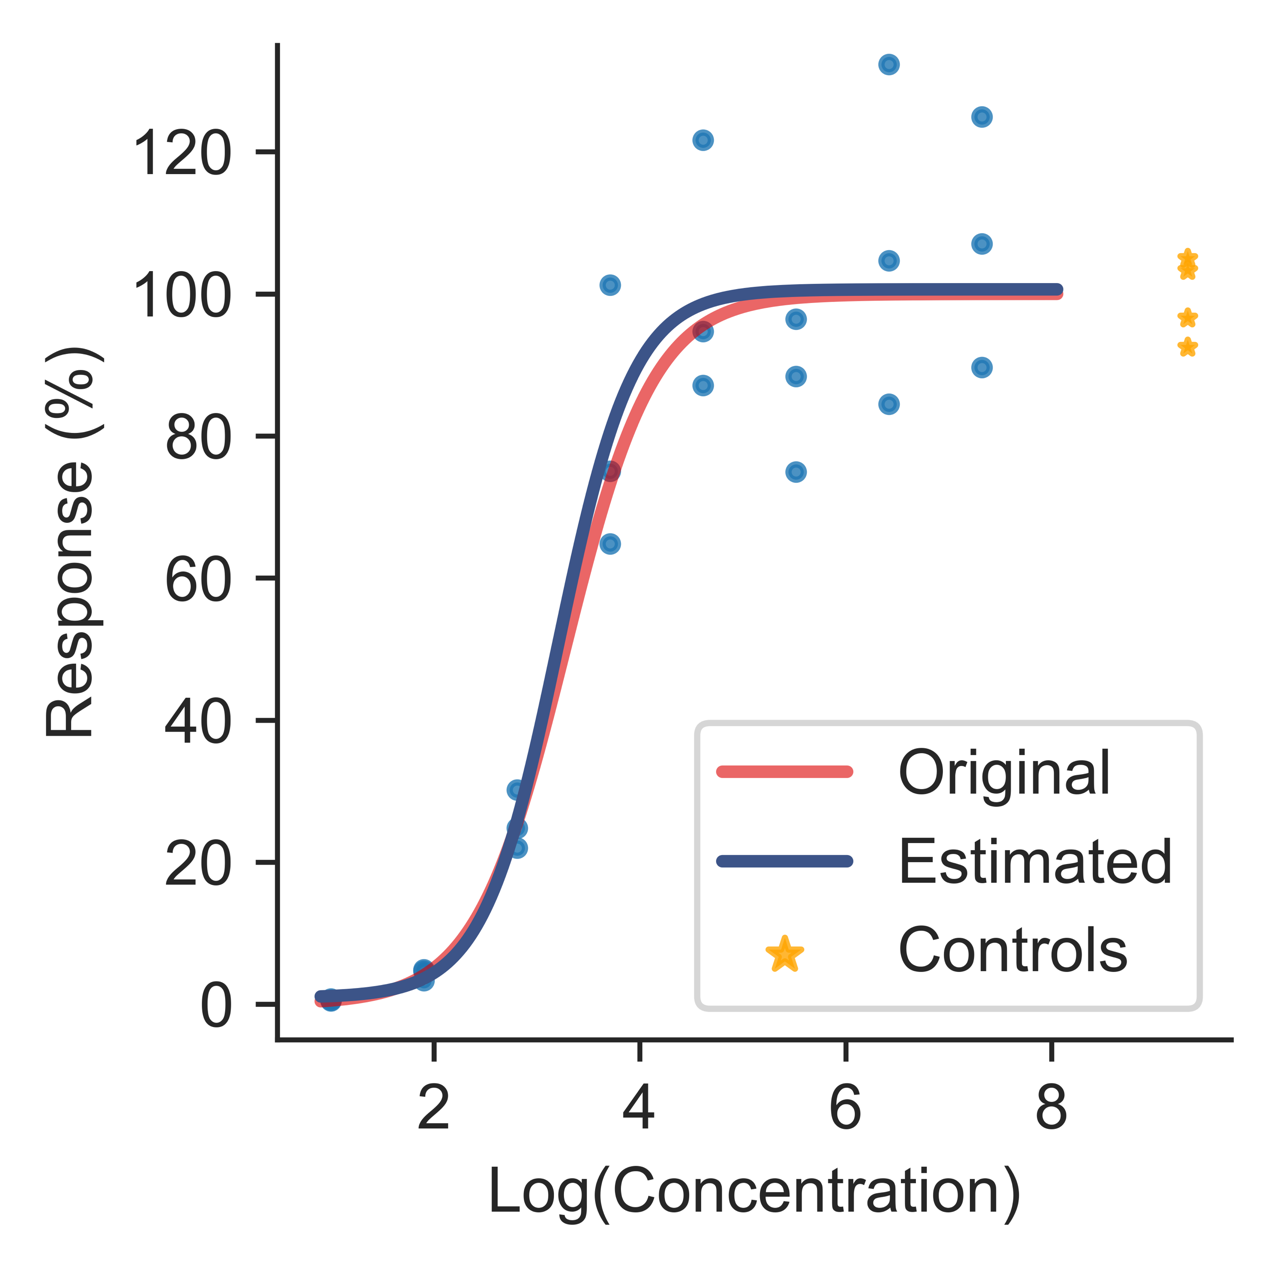
\includegraphics[width=0.9\textwidth]{figures/plate_layout_rand_02.npy_compound_1-right-half.png}
    \caption{$R^2=0.91$, $IC_{50}=61.92$}
    \label{fig:dr-borer-comp1}
  \end{subfigure}
  \hfill
  \begin{subfigure}[c]{0.3\textwidth}
    \centering
    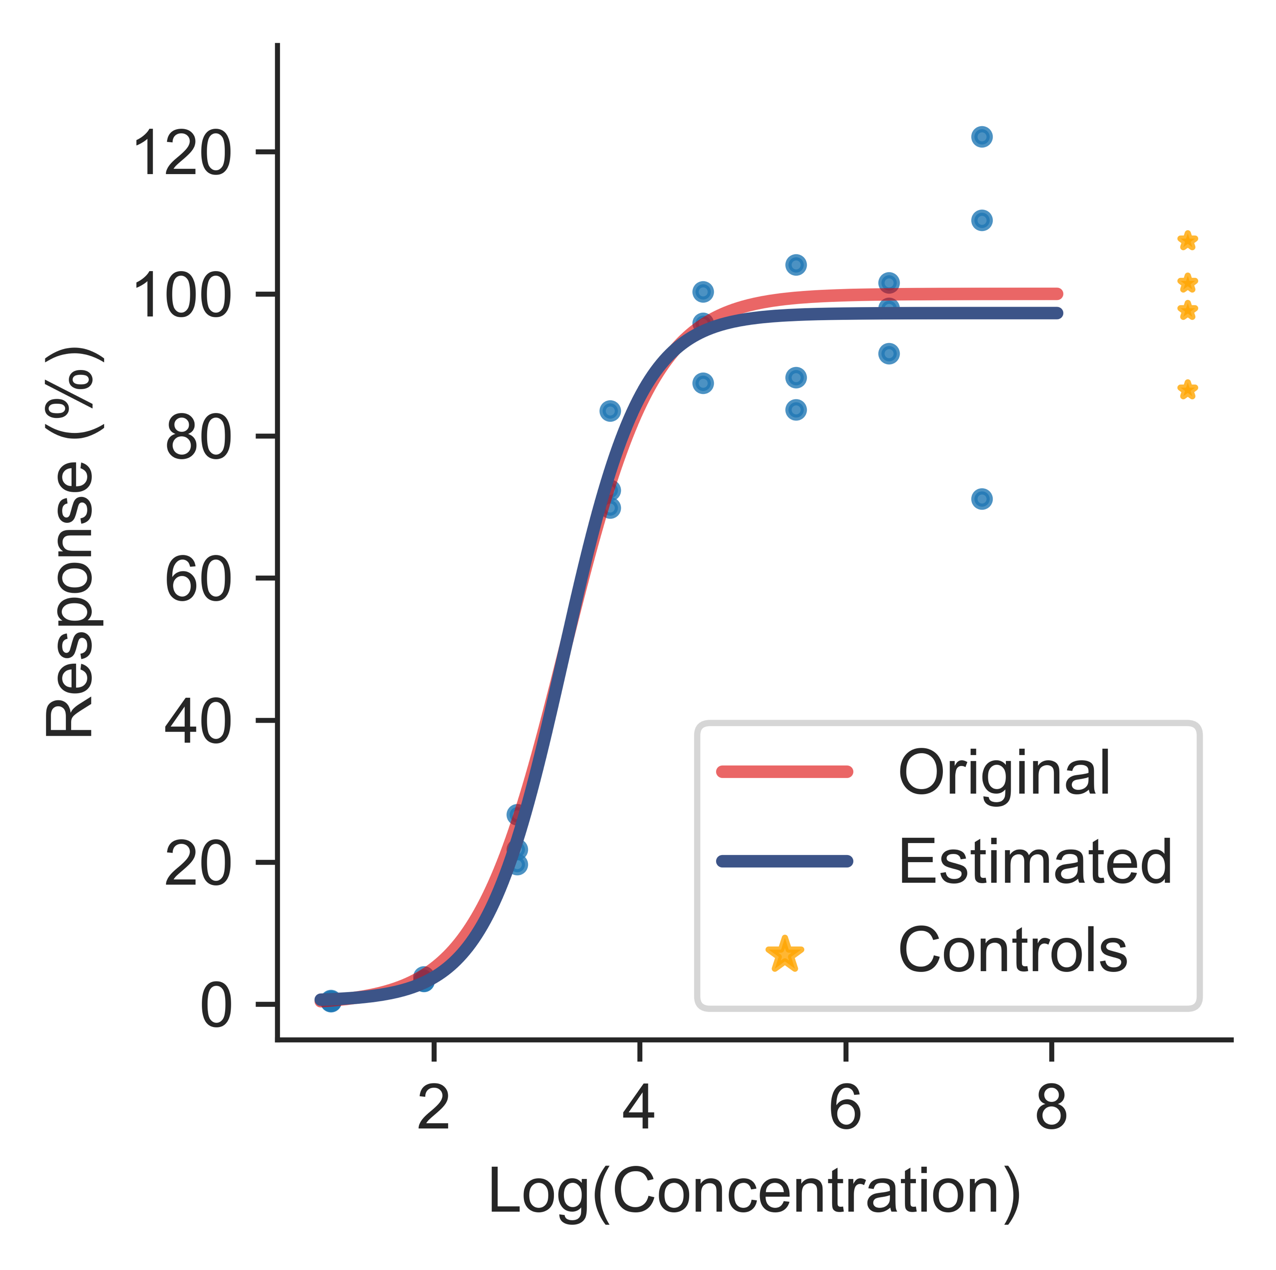
\includegraphics[width=0.9\textwidth]{figures/plate_layout_20-12-8-3_01.npy_compound_1-right-half.png}
    \caption{$R^2=0.95$, $IC_{50}=55.48$}
    \label{fig:dr-rand-comp1}
  \end{subfigure}
  \hfill
    \begin{subfigure}[c]{0.3\textwidth}
    \centering
    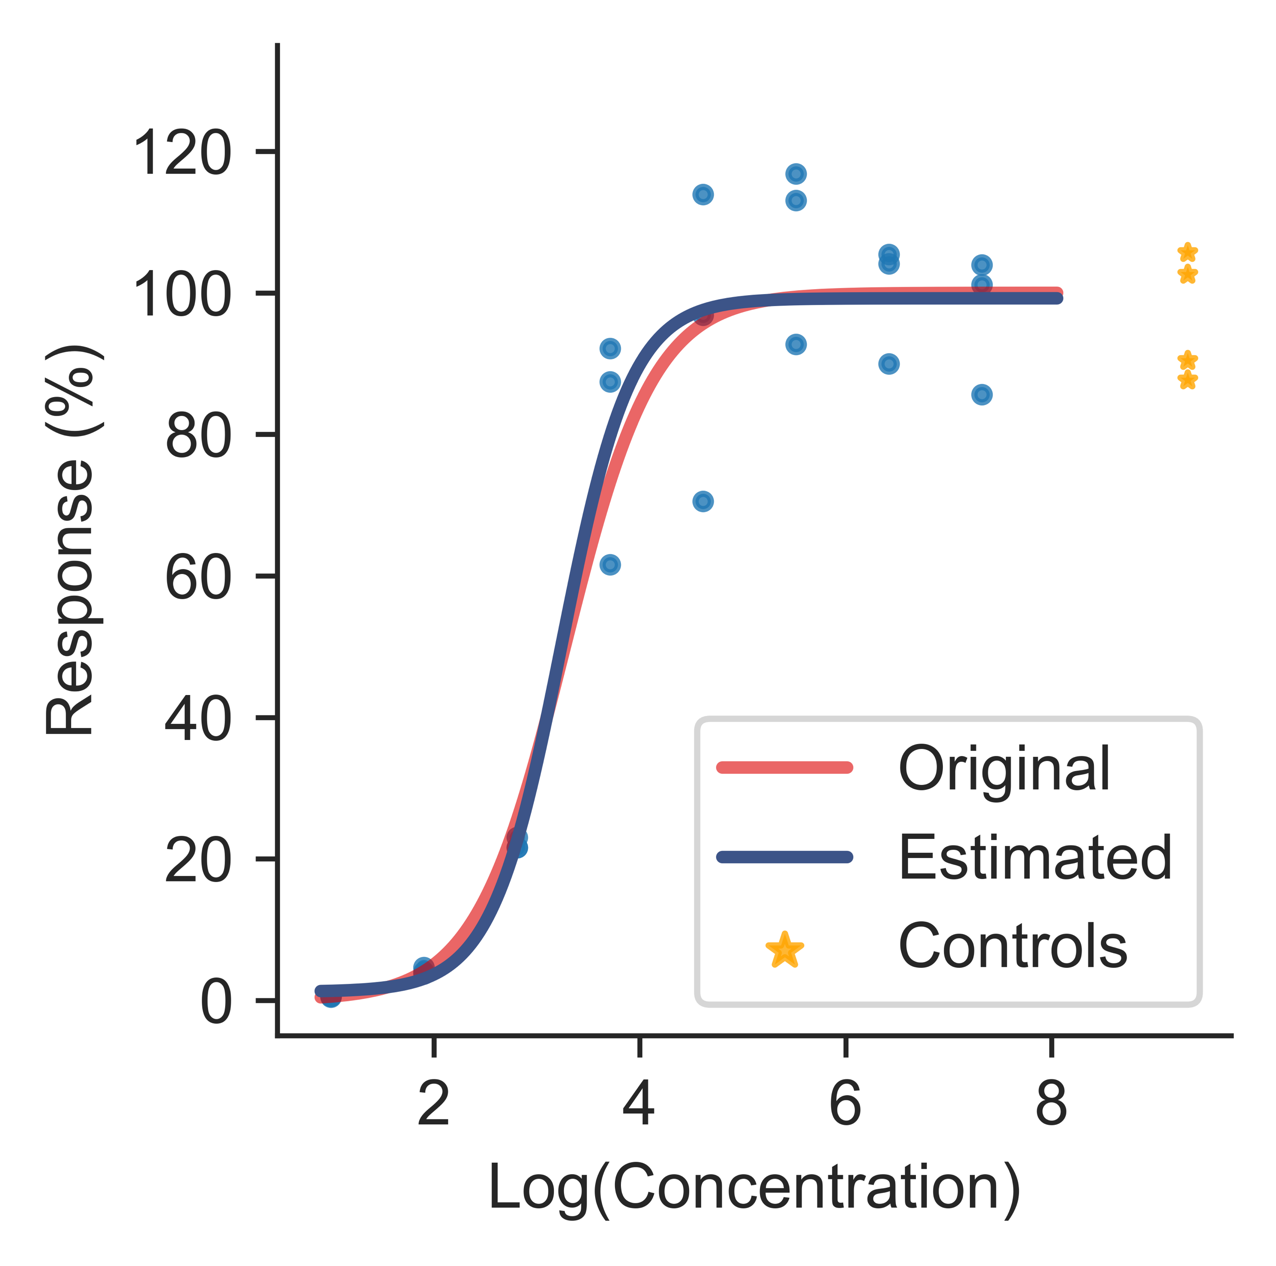
\includegraphics[width=0.9\textwidth]{figures/plate_layout_40-12-8-3_01.npy_compound_1-right-half.png}
    \caption{$R^2=0.95$, $IC_{50}=57.66$}
    \label{fig:dr-plaid-comp1}
  \end{subfigure}


  \vspace{5 mm}
  \begin{subfigure}[c]{0.05\textwidth}
    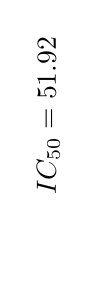
\begin{tikzpicture}
      \node[rotate=90] {~~~~~~~$IC_{50}=51.92$};  
    \end{tikzpicture}
  \end{subfigure}
  \hfill
  \begin{subfigure}[c]{0.3\textwidth}
    \centering
    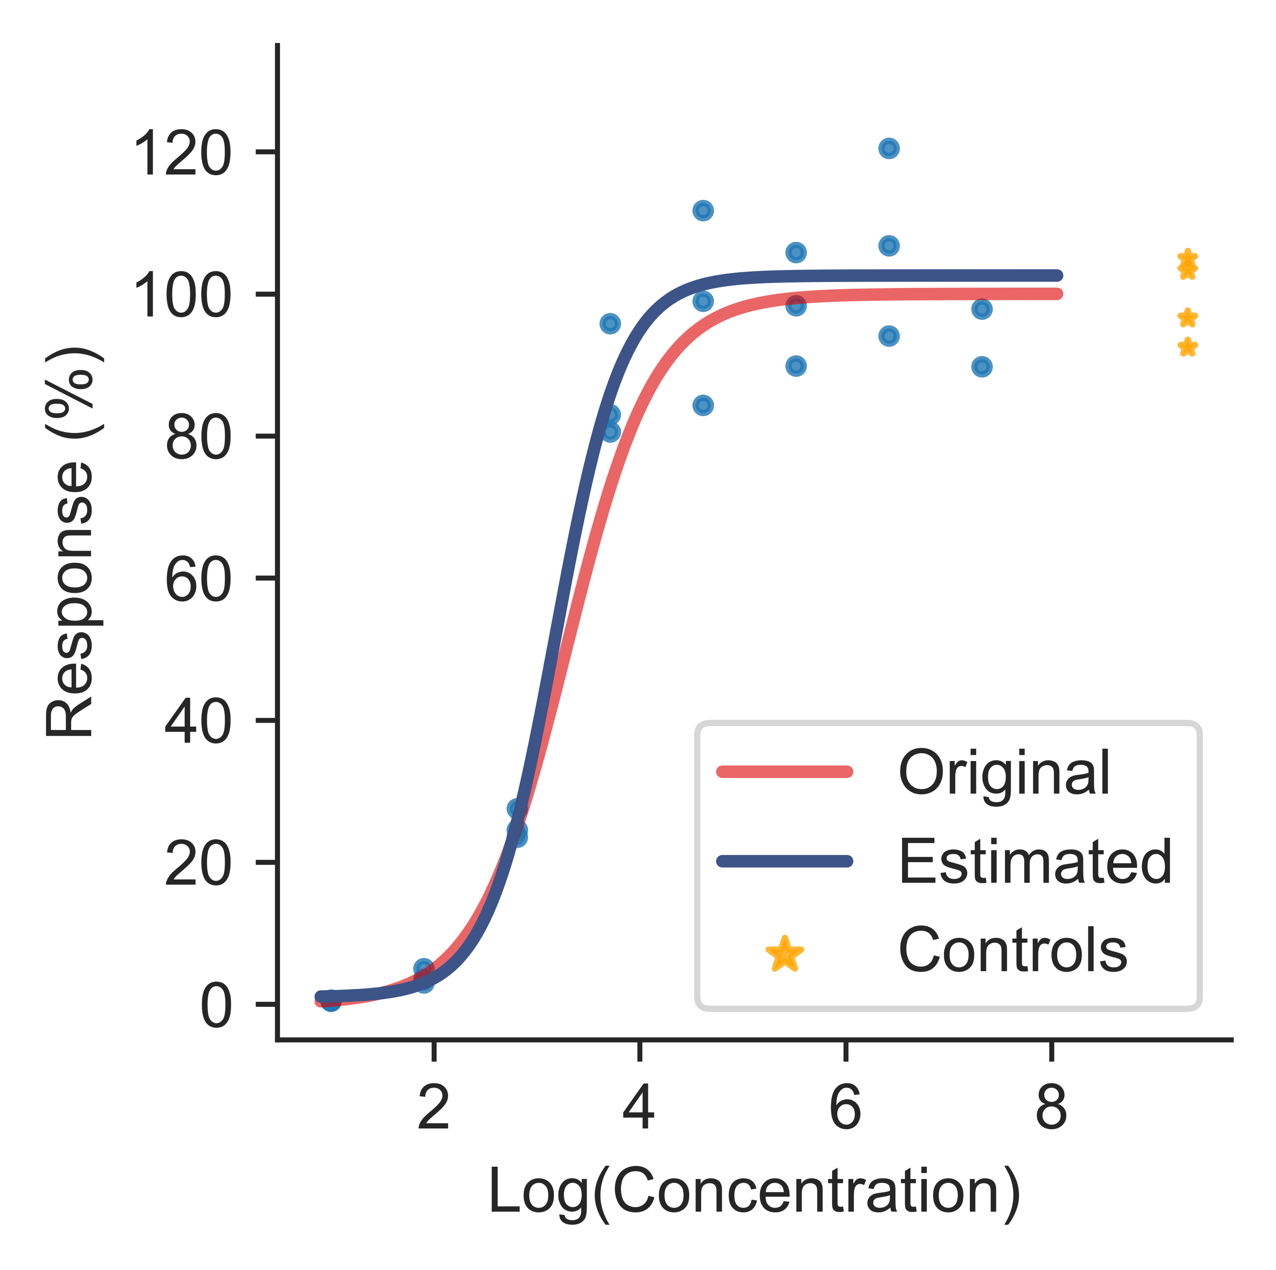
\includegraphics[width=0.9\textwidth]{figures/plate_layout_rand_02.npy_compound_4-right-half.png}
    \caption{$R^2=0.95$, $IC_{50}=66.16$}
    \label{fig:dr-border-comp5}
  \end{subfigure} 
  \hfill
  \begin{subfigure}[c]{0.3\textwidth}
    \centering
    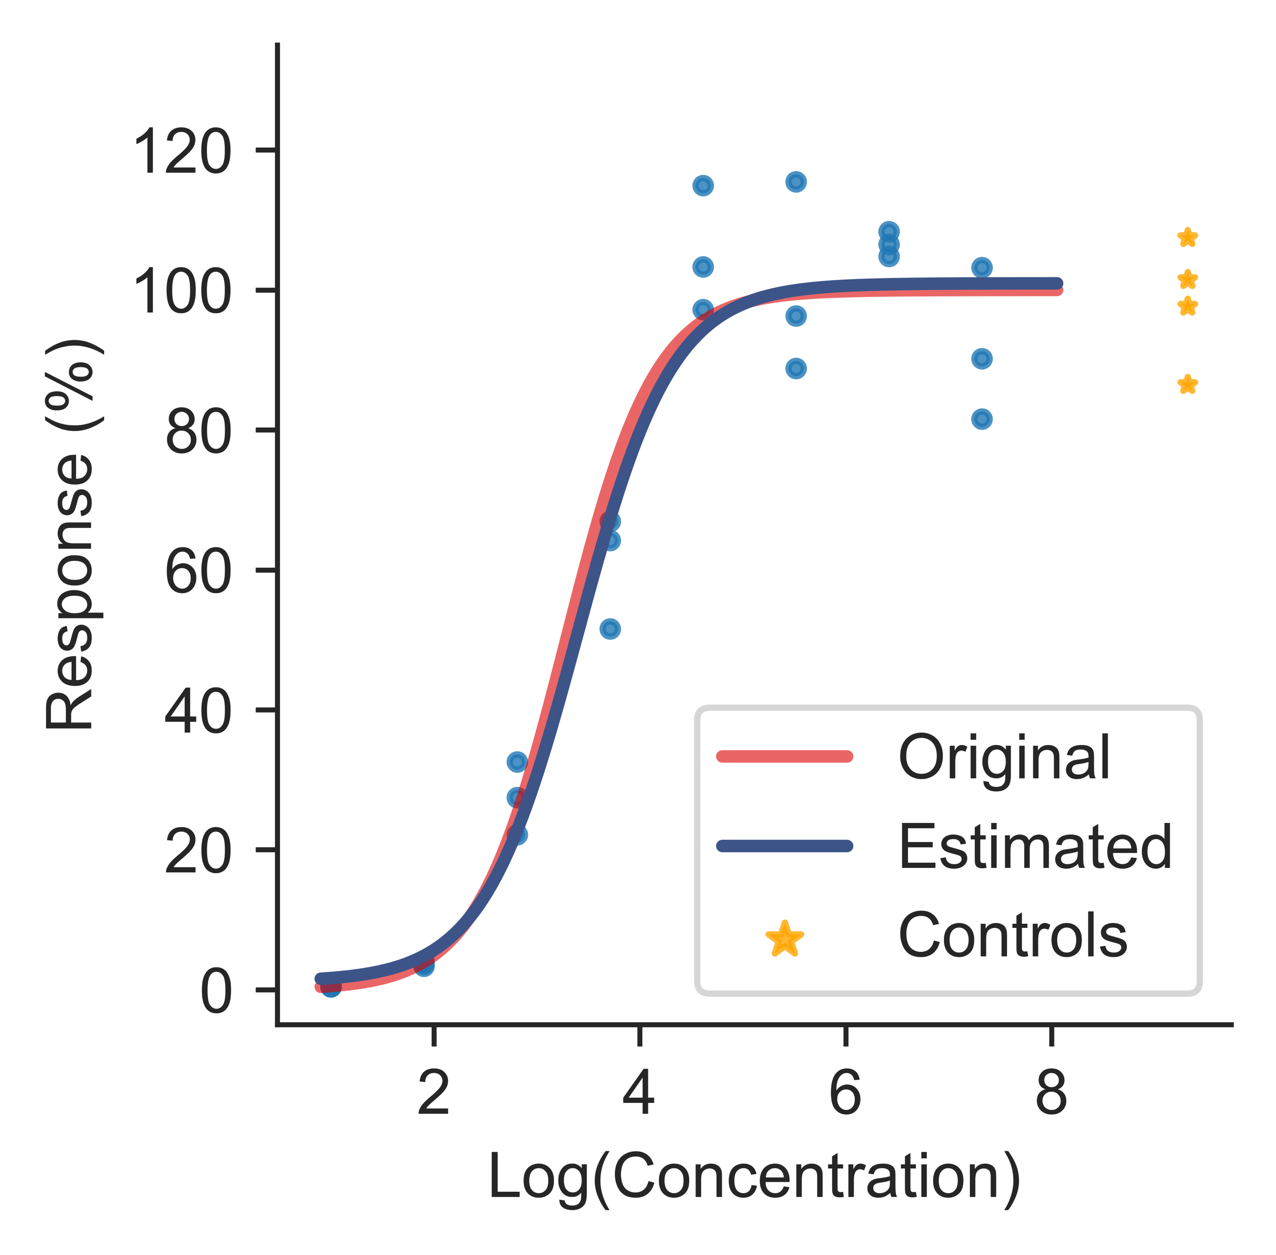
\includegraphics[width=0.9\textwidth]{figures/plate_layout_20-12-8-3_01.npy_compound_4-right-half.png}
    \caption{$R^2=0.96$, $IC_{50}=39.99$}
    \label{fig:dr-random-comp5}
  \end{subfigure}
      \hfill
    \begin{subfigure}[c]{0.3\textwidth}
    \centering
    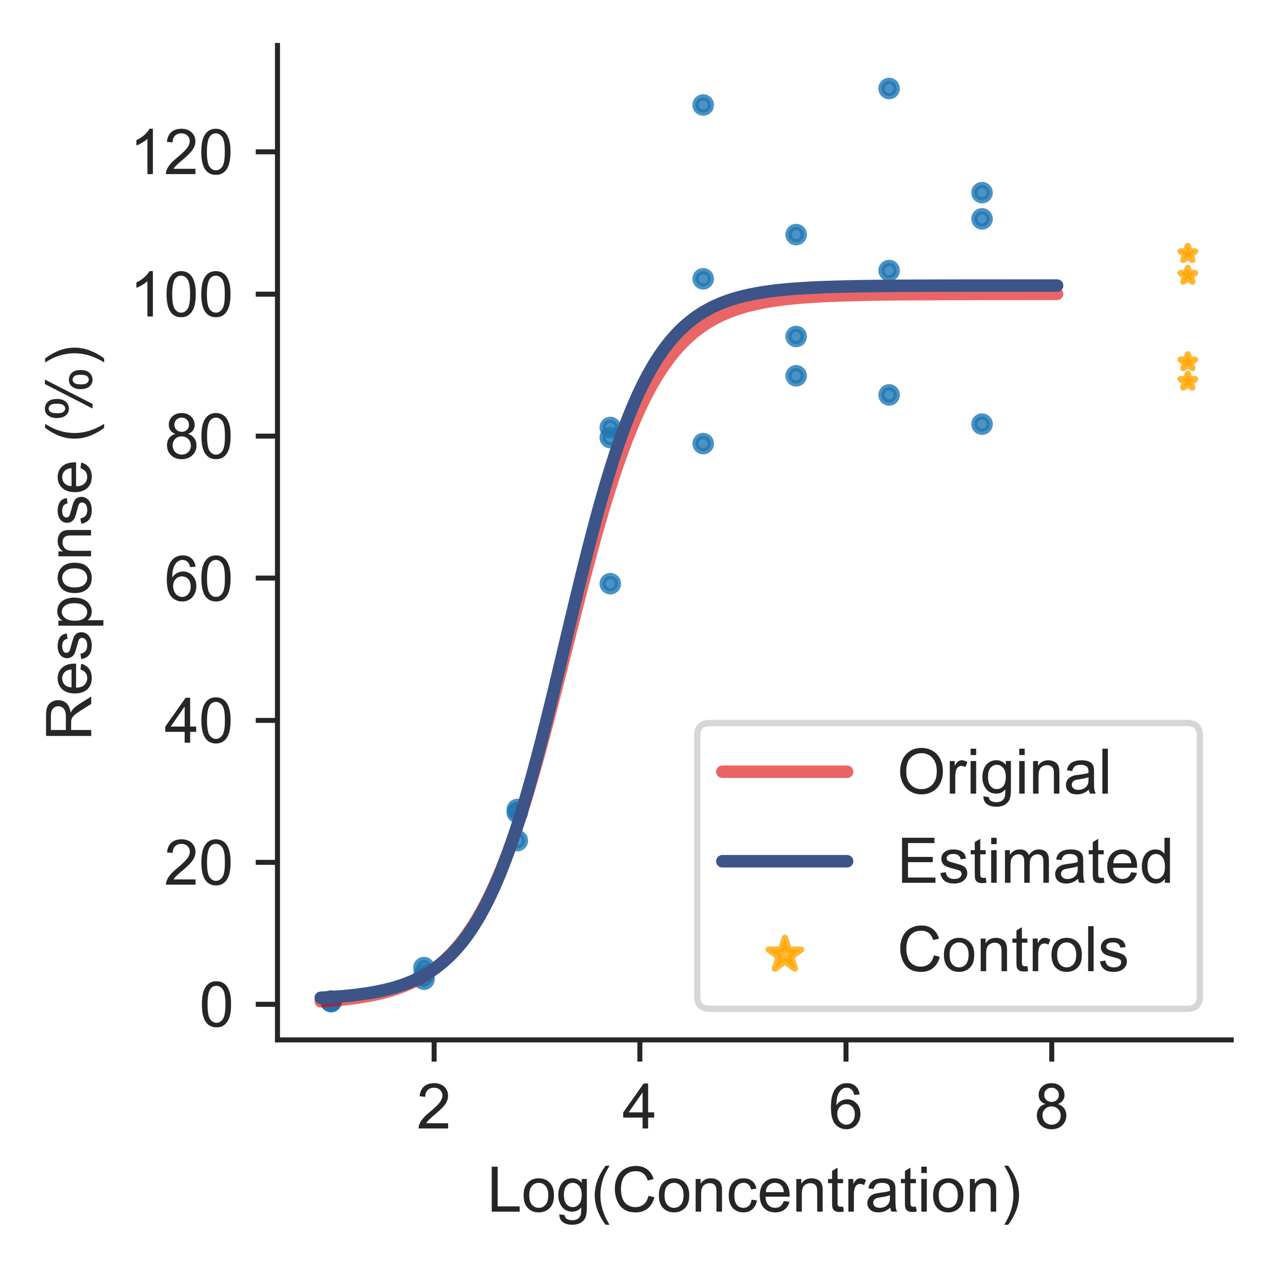
\includegraphics[width=0.9\textwidth]{figures/plate_layout_40-12-8-3_01.npy_compound_4-right-half.png}
    \caption{$R^2=0.93$, $IC_{50}=53.02$}
    \label{fig:dr-plaid-comp5}
  \end{subfigure}




  \vspace{5 mm}
  \begin{subfigure}[c]{0.05\textwidth}
    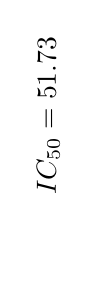
\begin{tikzpicture}
      \node[rotate=90] {~~~~~~~$IC_{50}=51.73$};  
    \end{tikzpicture}
  \end{subfigure}  
  \hfill
  \begin{subfigure}[c]{0.3\textwidth}
    \centering
    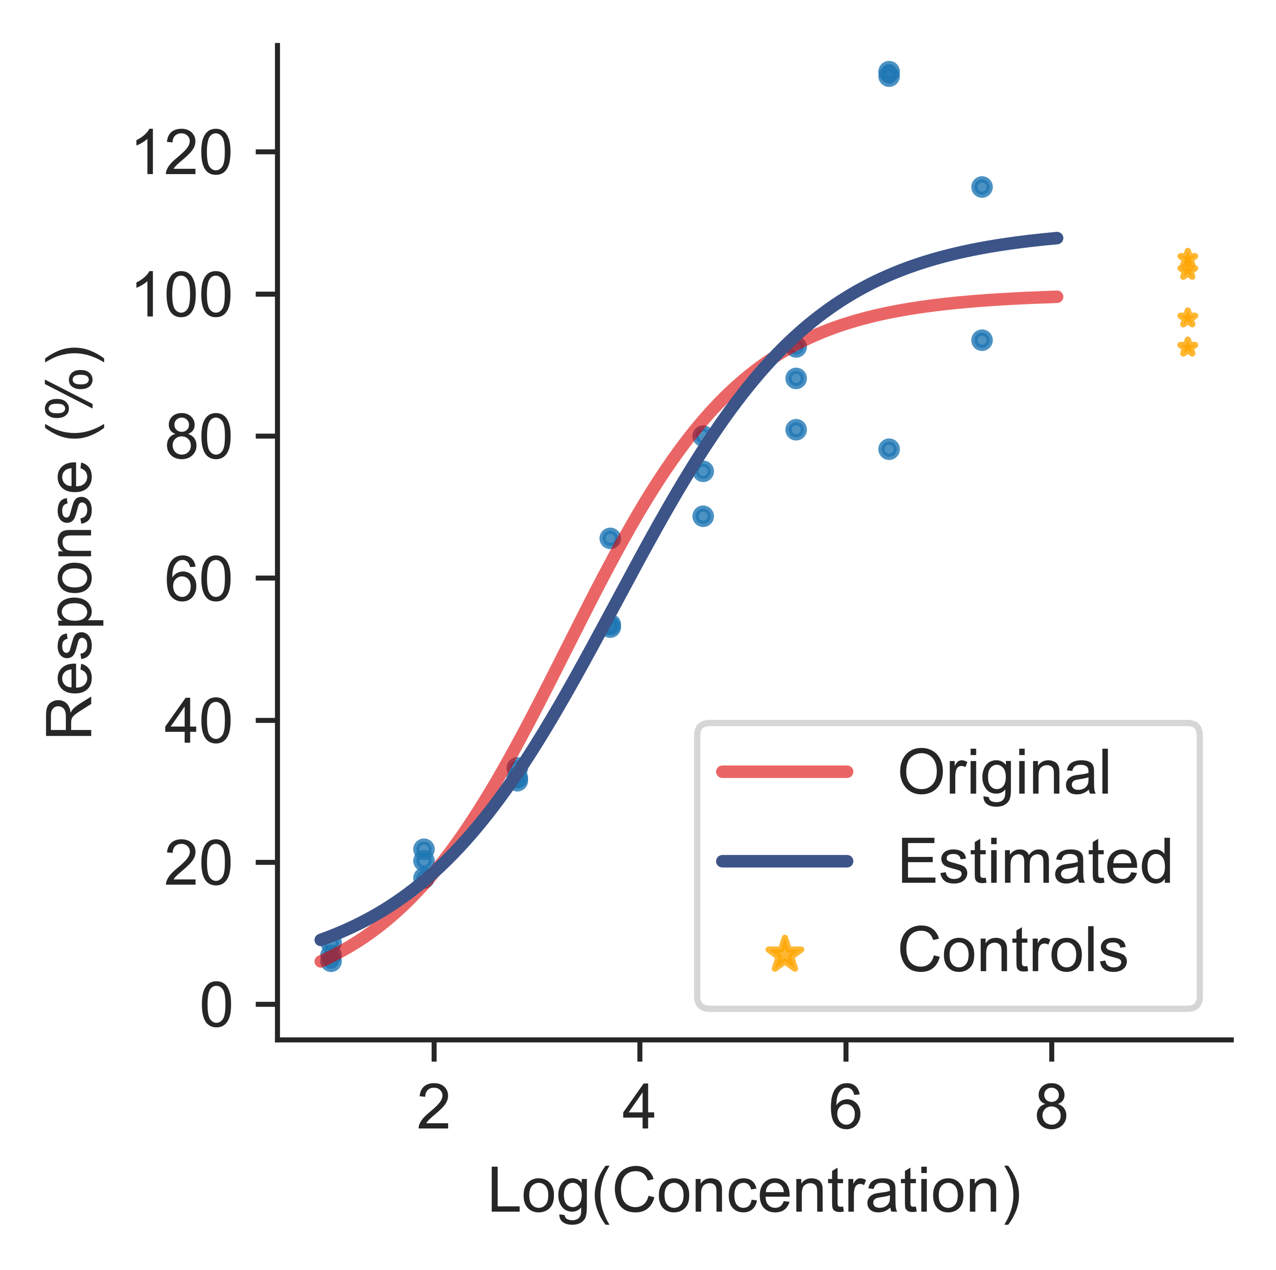
\includegraphics[width=0.9\textwidth]{figures/plate_layout_rand_02.npy_compound_9-right-half.png}
    \caption{$R^2=0.90$, $IC_{50}=17.19$}
    \label{fig:dr-border-comp9}
  \end{subfigure}
  \hfill
  \begin{subfigure}[c]{0.3\textwidth}
    \centering
    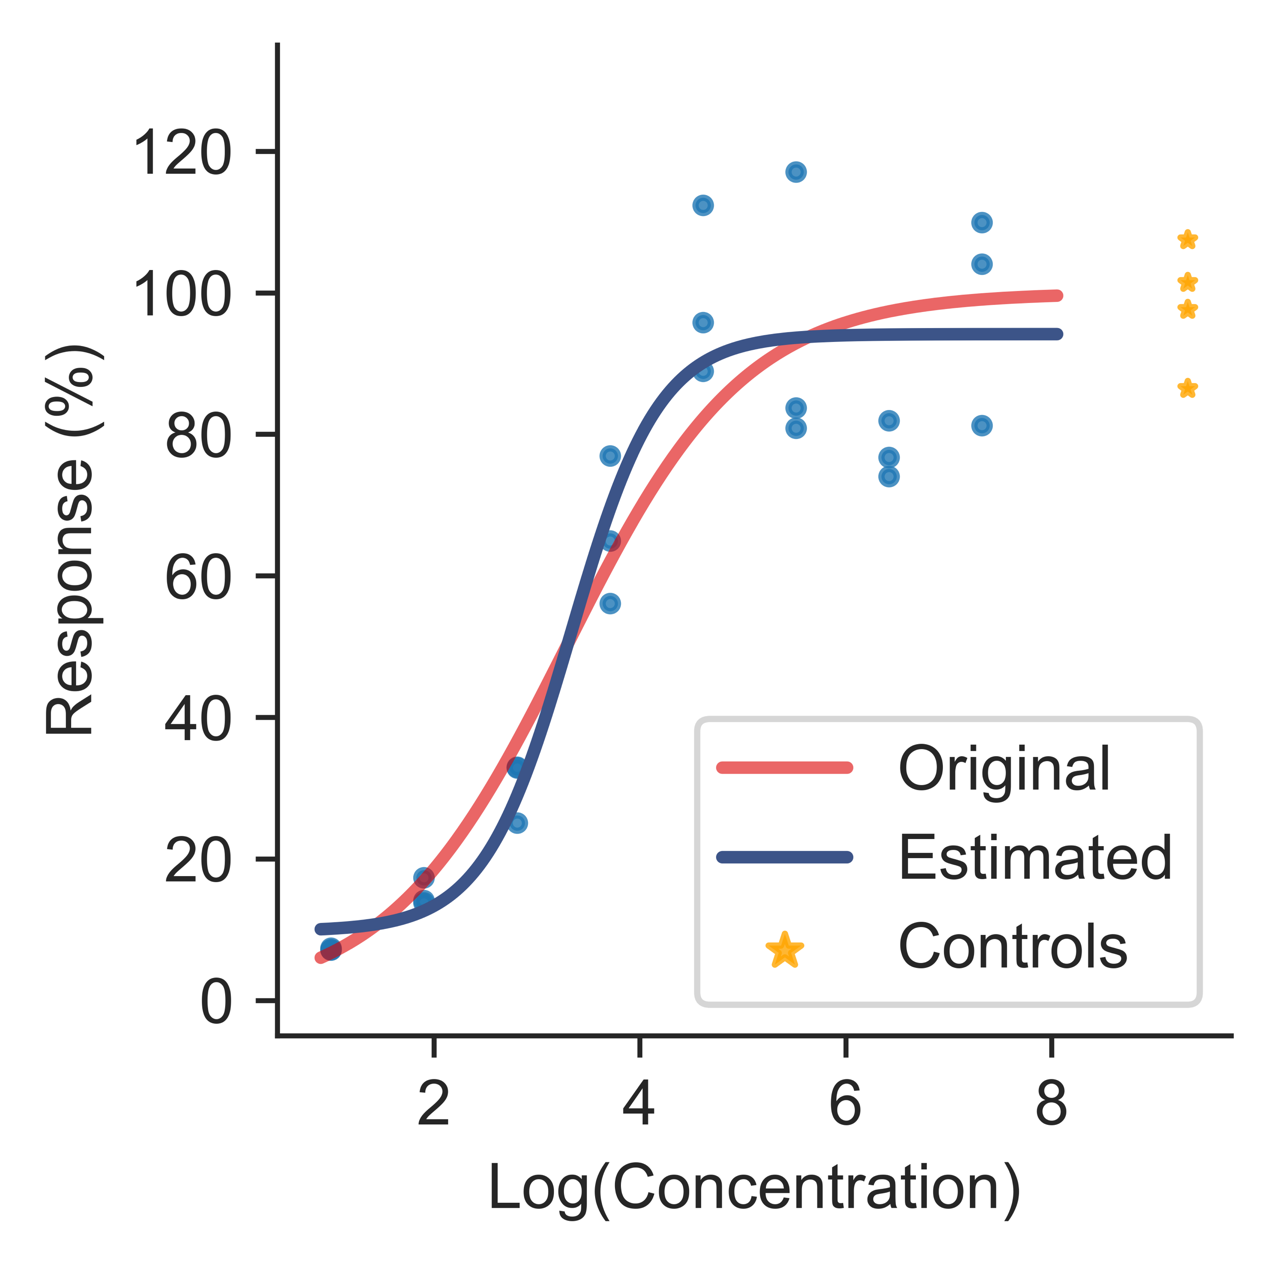
\includegraphics[width=0.9\textwidth]{figures/plate_layout_20-12-8-3_01.npy_compound_9-right-half.png}
    \caption{$R^2=0.91$, $IC_{50}=46.57$}
    \label{fig:dr-random-comp9}
  \end{subfigure}
  \hfill
    \begin{subfigure}[c]{0.3\textwidth}
    \centering
    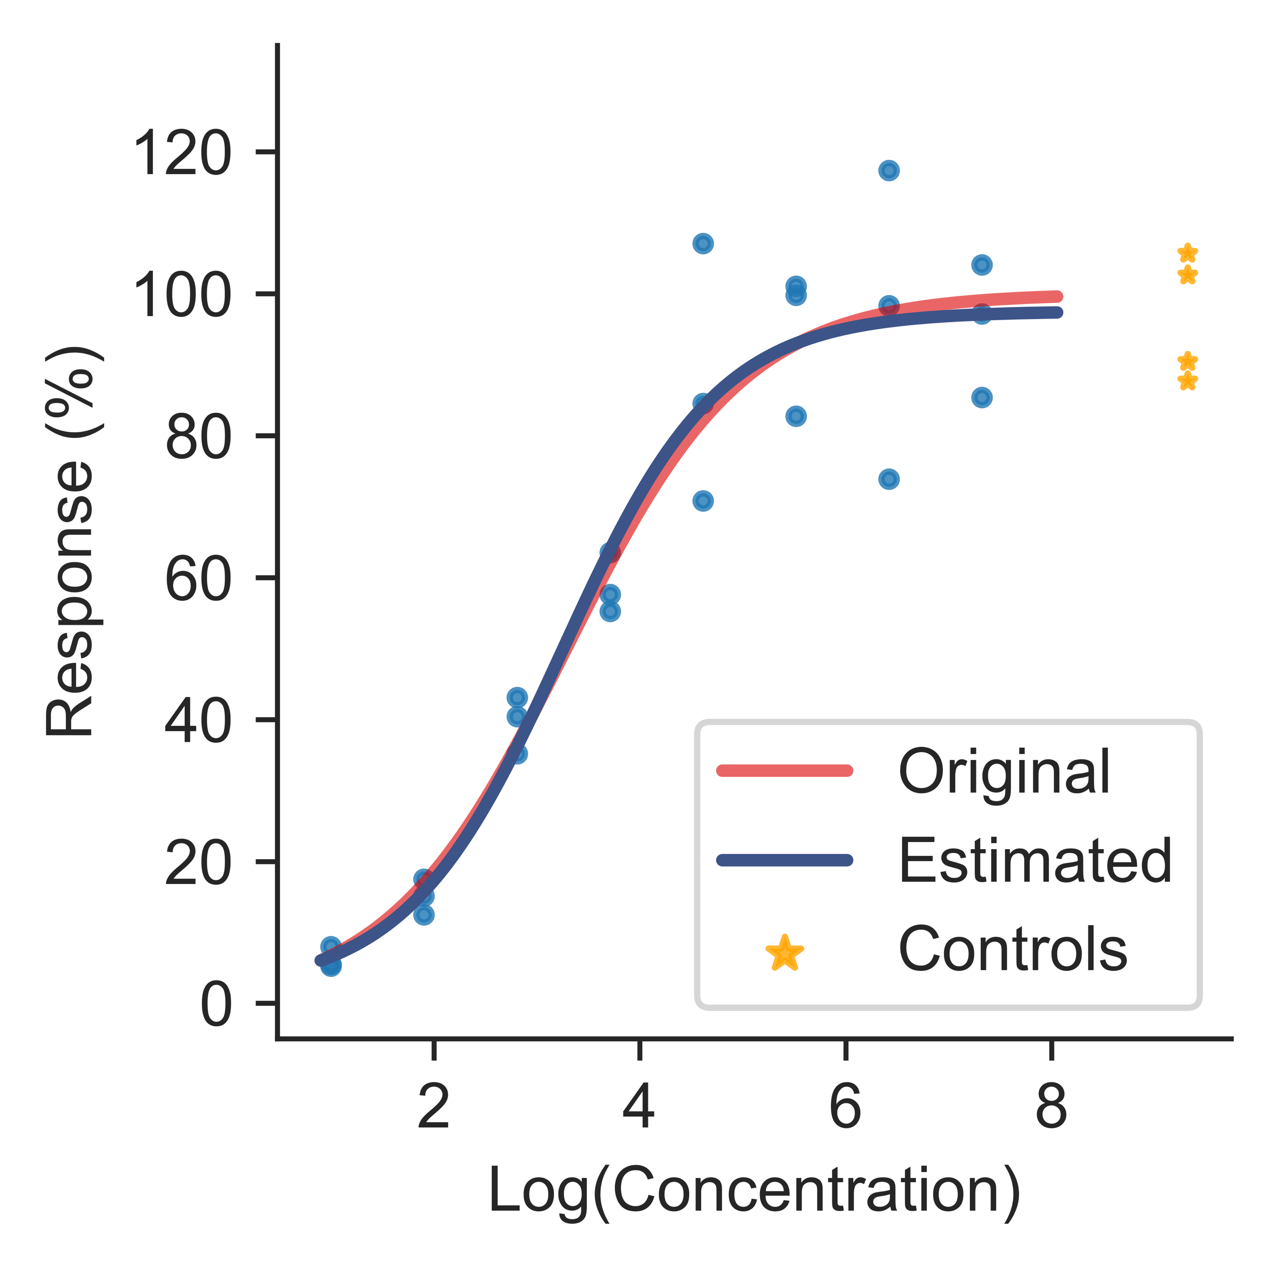
\includegraphics[width=0.9\textwidth]{figures/plate_layout_40-12-8-3_01.npy_compound_9-right-half.png}
    \caption{$R^2=0.93$, $IC_{50}=56.59$}
    \label{fig:dr-plaid-comp9}
  \end{subfigure}


  \caption{Examples of dose response curves for simulated experiments
    using 8~doses with 3~replicates (blue dots), 4~negative controls
    (yellow stars), and strong bowl-shaped plate effects. On the left
    of each row we show the expected $IC_{50}$ value. On the caption
    below each plot we show the obtained $R^2$ and $IC_{50}$ values.}
  \label{fig:dose-response-curves} 
\end{figure*}








%%% Local Variables: 
%%% mode: latex
%%% TeX-master: "../supplement.tex"
%%% End: 